\section{System Components}
The system is composed of two main components: the front-end and the back-end,
which work together to provide a seamless user experience and efficient data processing.

\subsection{Frontend Components}
The front-end of the system is built using Next.js, a React-based framework that
enables server-side rendering and static site generation for improved performance.
This component is responsible for the user interface, allowing patients and administrators
to interact with the system. Users can register, log in, submit their medical data, and view
their prediction results through a responsive and intuitive interface. Administrators,
on the other hand, have access to dashboards where they can view predictions submitted by all users.
The front-end communicates with the back-end through RESTful APIs,
ensuring that user actions are efficiently processed and results are delivered in real time.
\subsection{Backend Components}
The back-end of the system is implemented using FastAPI\footnote{\url{https://fastapi.tiangolo.com/}} 
, a modern Python framework
designed for high-performance APIs. This component handles authentication, authorization,
and data management. It processes user-submitted medical data,
forwards the input to the pre-trained machine learning model built with Scikit-Learn,
and returns prediction results to the front-end. The back-end also manages the storage and retrieval
of user data and prediction records using a relational database, implemented with SQLite for simplicity and reliability.
Furthermore, Docker is used to containerize the application, ensuring consistency across development and deployment environments.

Together, the front-end and back-end form a robust system that supports medical prediction tasks,
ensuring usability, performance, and scalability for both patients and administrators.
\subsection{Dataflow Diagram}
\begin{figure}[htbp]
  \begin{center}
    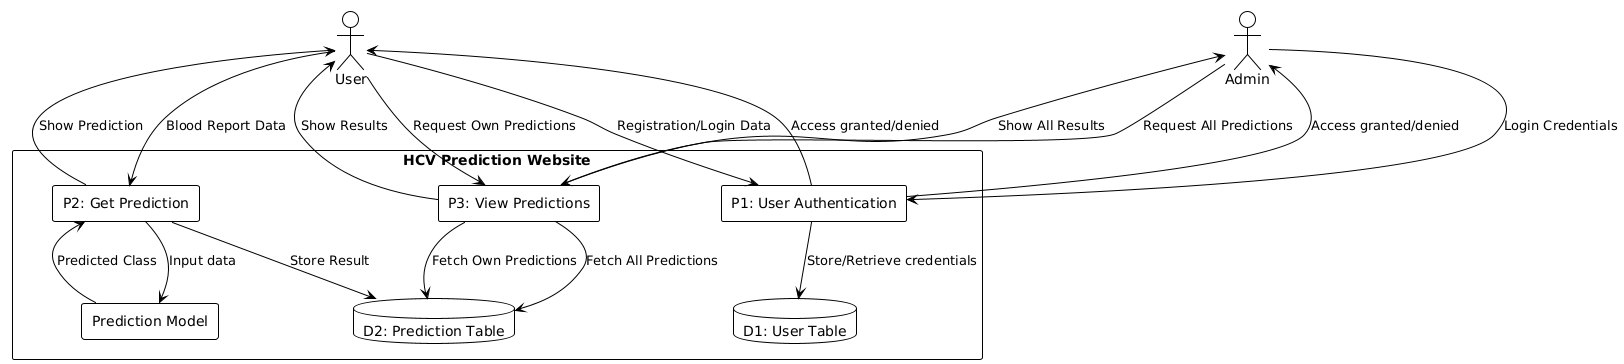
\includegraphics[width=\textwidth]{figures/dataflow.png}
  \end{center}
  \caption{Dataflow diagram of the website}\label{fig:dataflow}
\end{figure}

\subsection{Sequence Diagram}

\begin{figure}[htbp]
  \begin{center}
    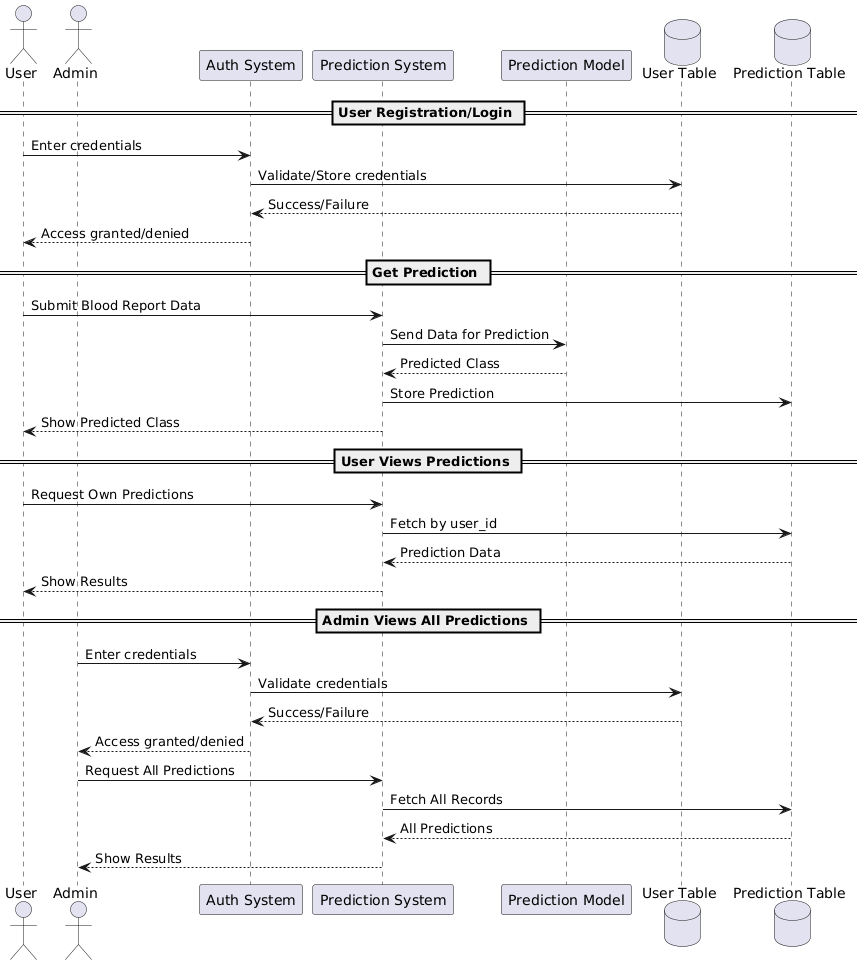
\includegraphics[width=\textwidth]{figures/sequence-diagram.png}
  \end{center}
  \caption{Sequence diagram for showing how the user interacts with the website}\label{fig:sequence-diagram}
\end{figure}

\subsection{Key Features \& Page Screenshots}

\begin{figure}
  \begin{center}
    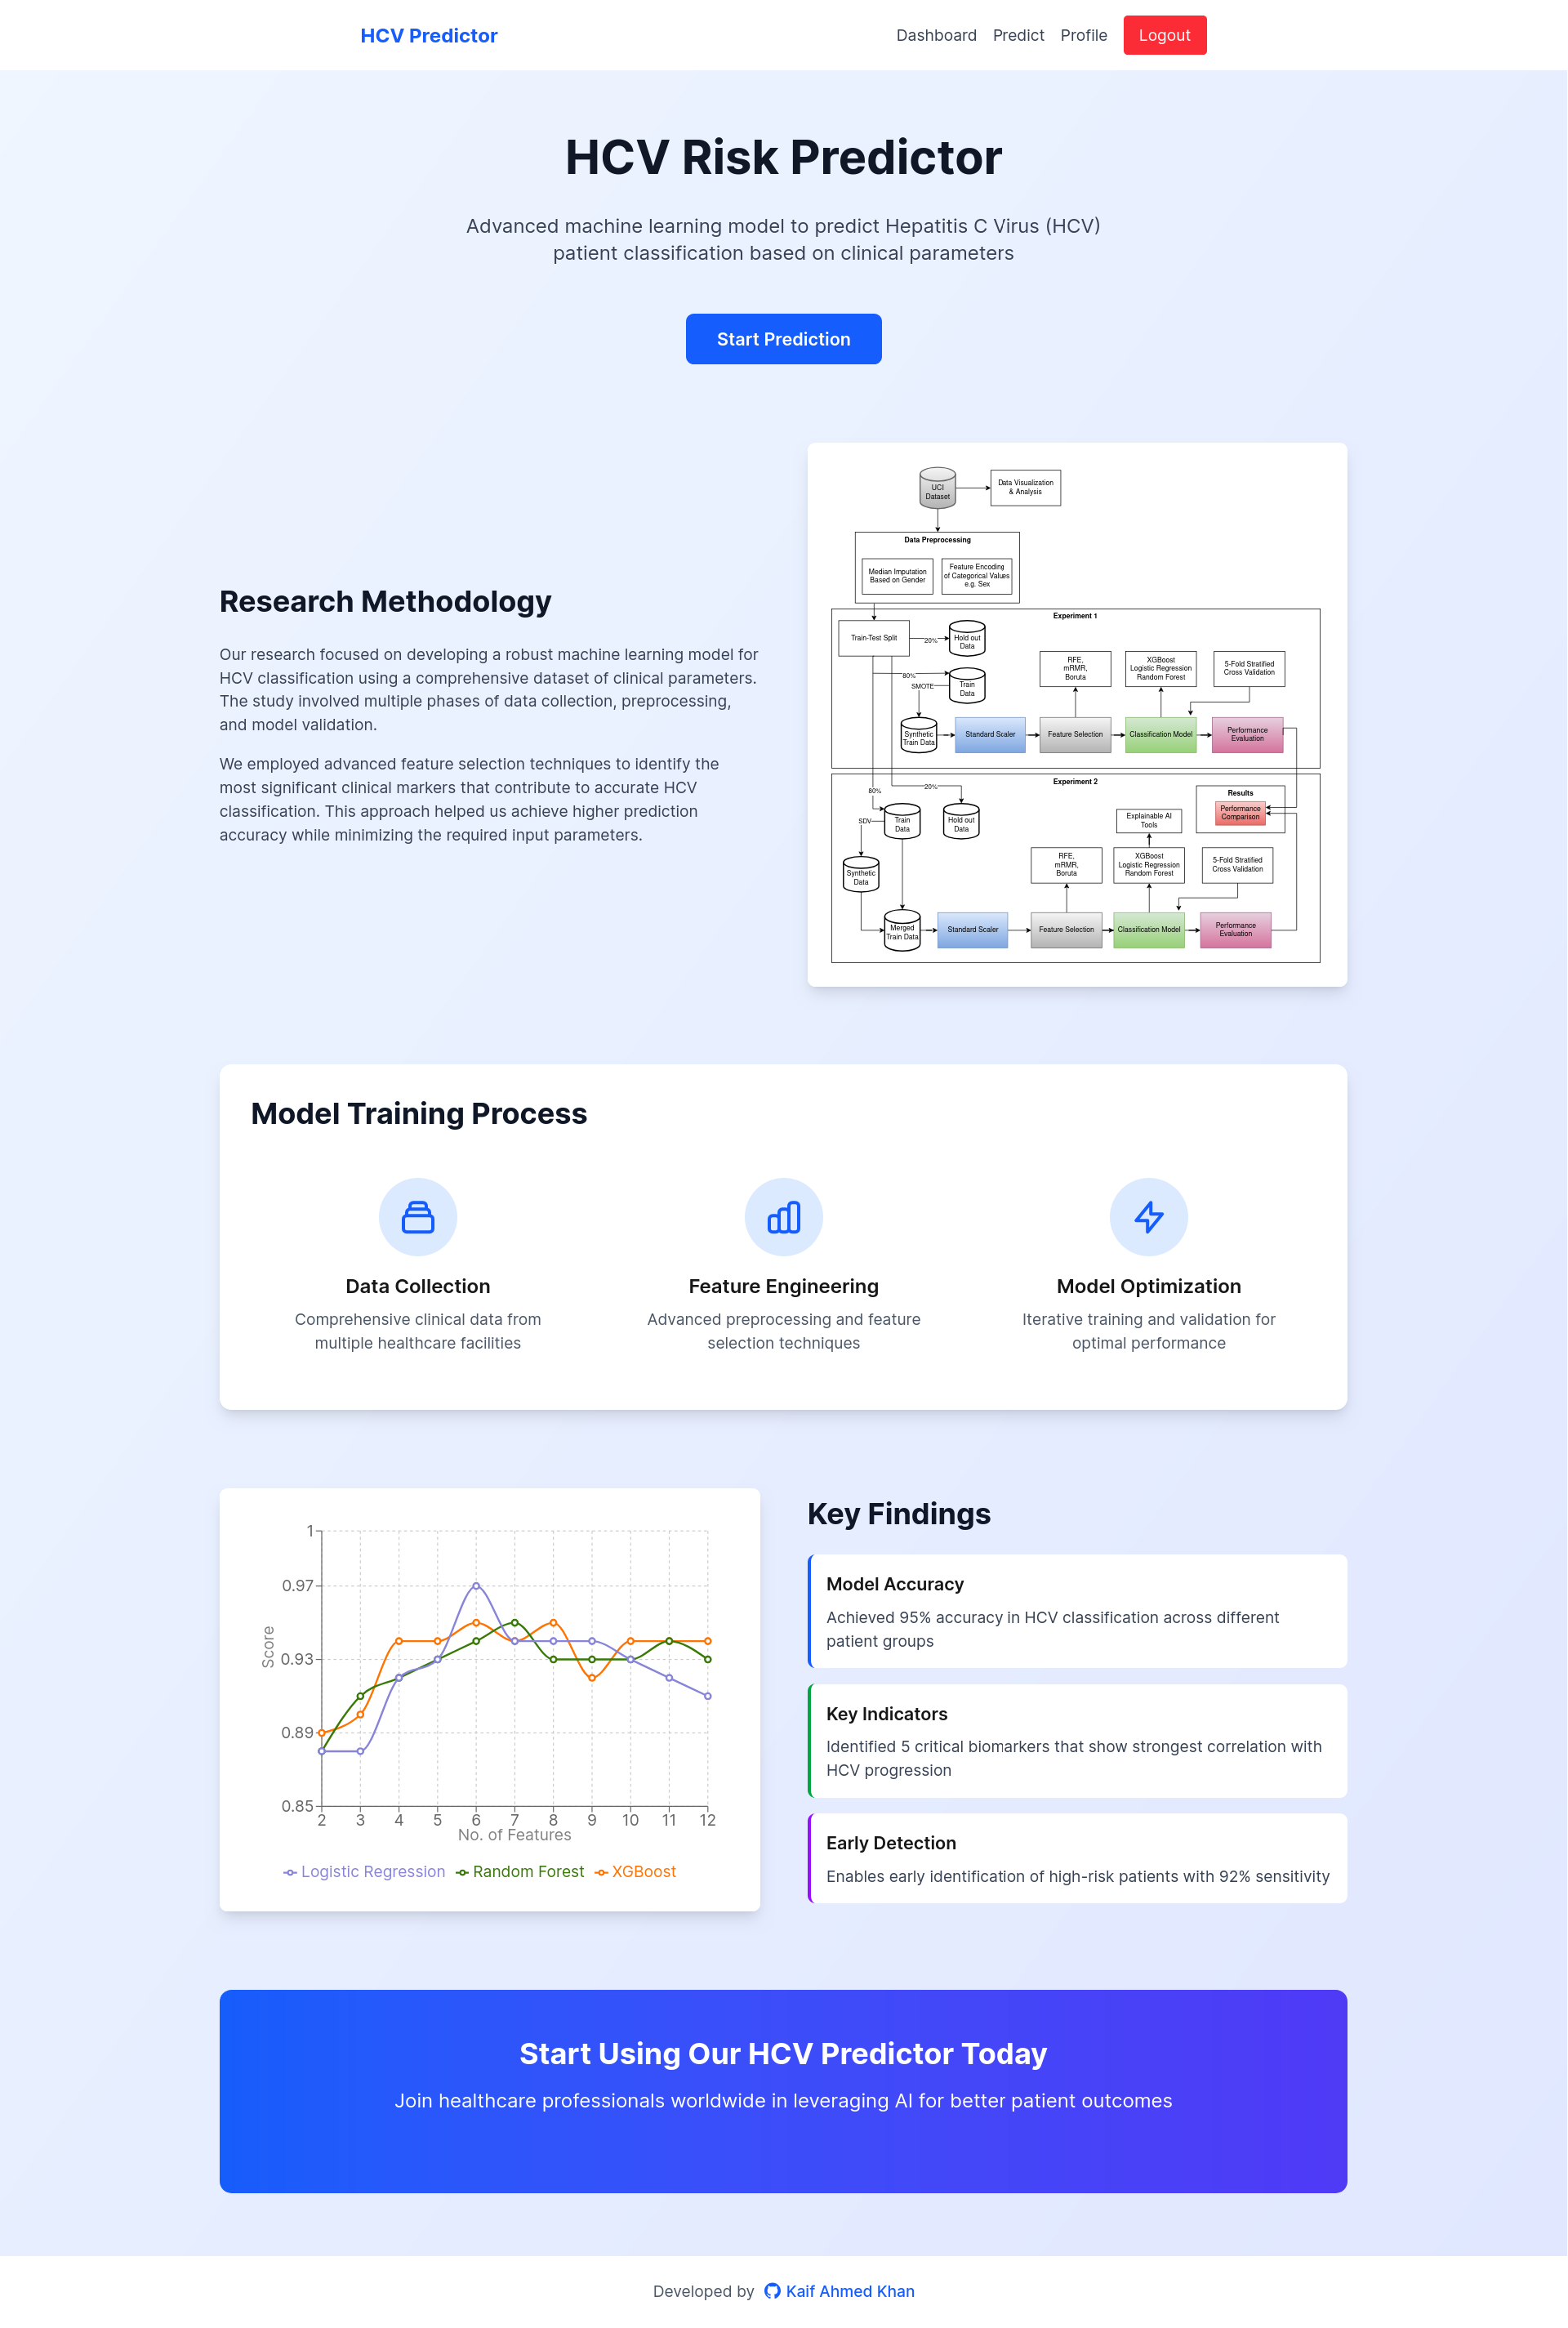
\includegraphics[width=0.95\textwidth]{figures/site/homepage.png}
  \end{center}
  \caption{Homepage of HCV Predictor}\label{fig:homepage}
\end{figure}


\begin{figure}[htbp]
  \begin{subfigure}{0.5\textwidth}
    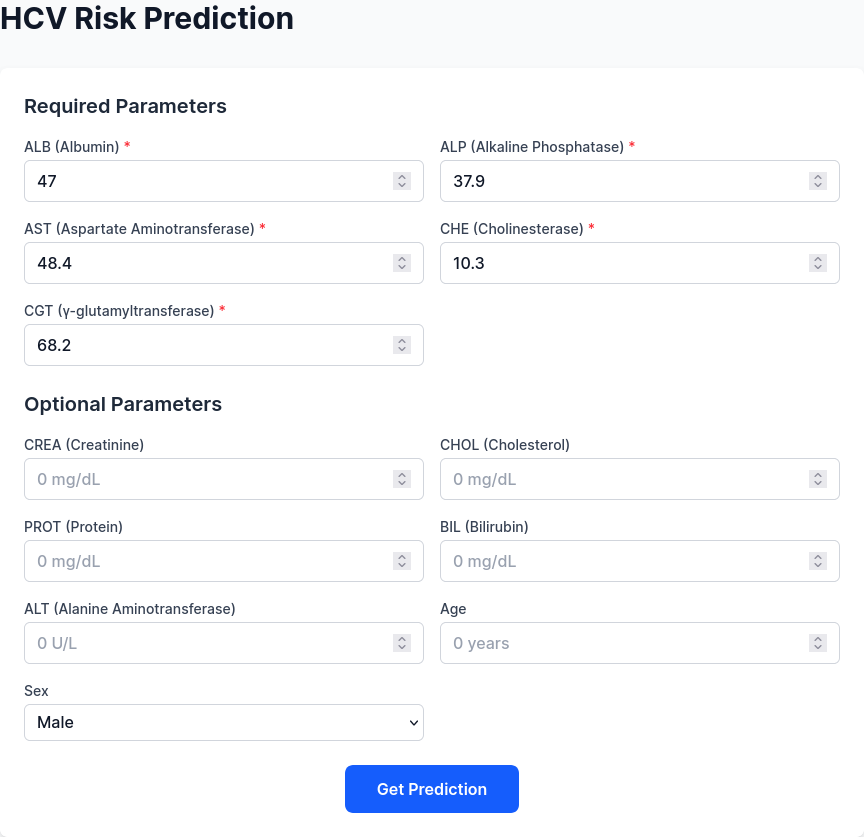
\includegraphics[width=\textwidth]{figures/site/predict1.png} 
    \caption{Prediction form}
    \label{fig:form}
  \end{subfigure}
  \begin{subfigure}{0.5\textwidth}
    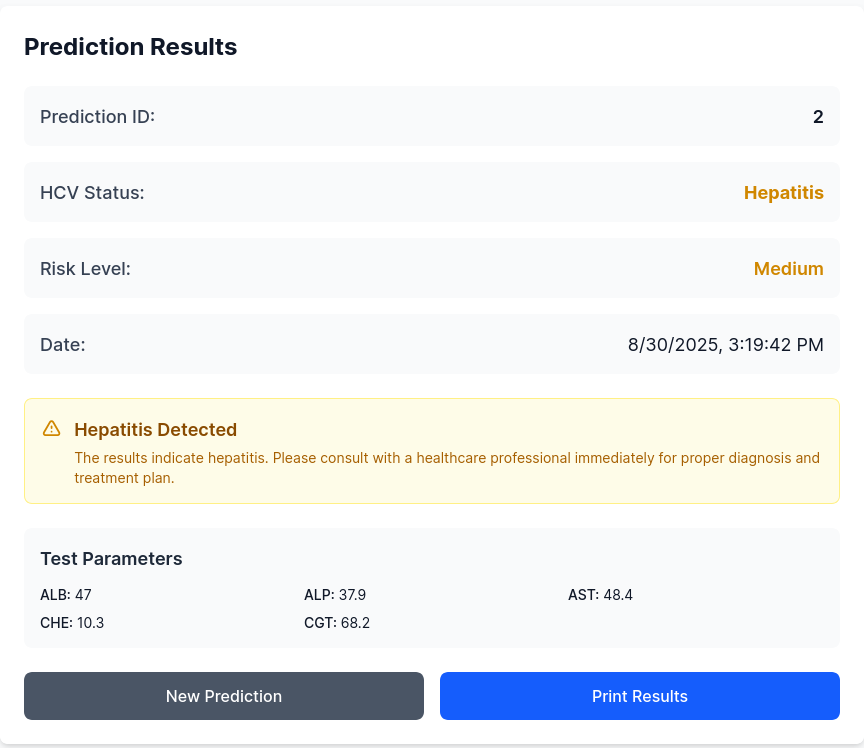
\includegraphics[width=\textwidth]{figures/site/predict2.png}
    \caption{Prediction result}
    \label{fig:prediction}
  \end{subfigure}
  \begin{subfigure}{0.5\textwidth}
    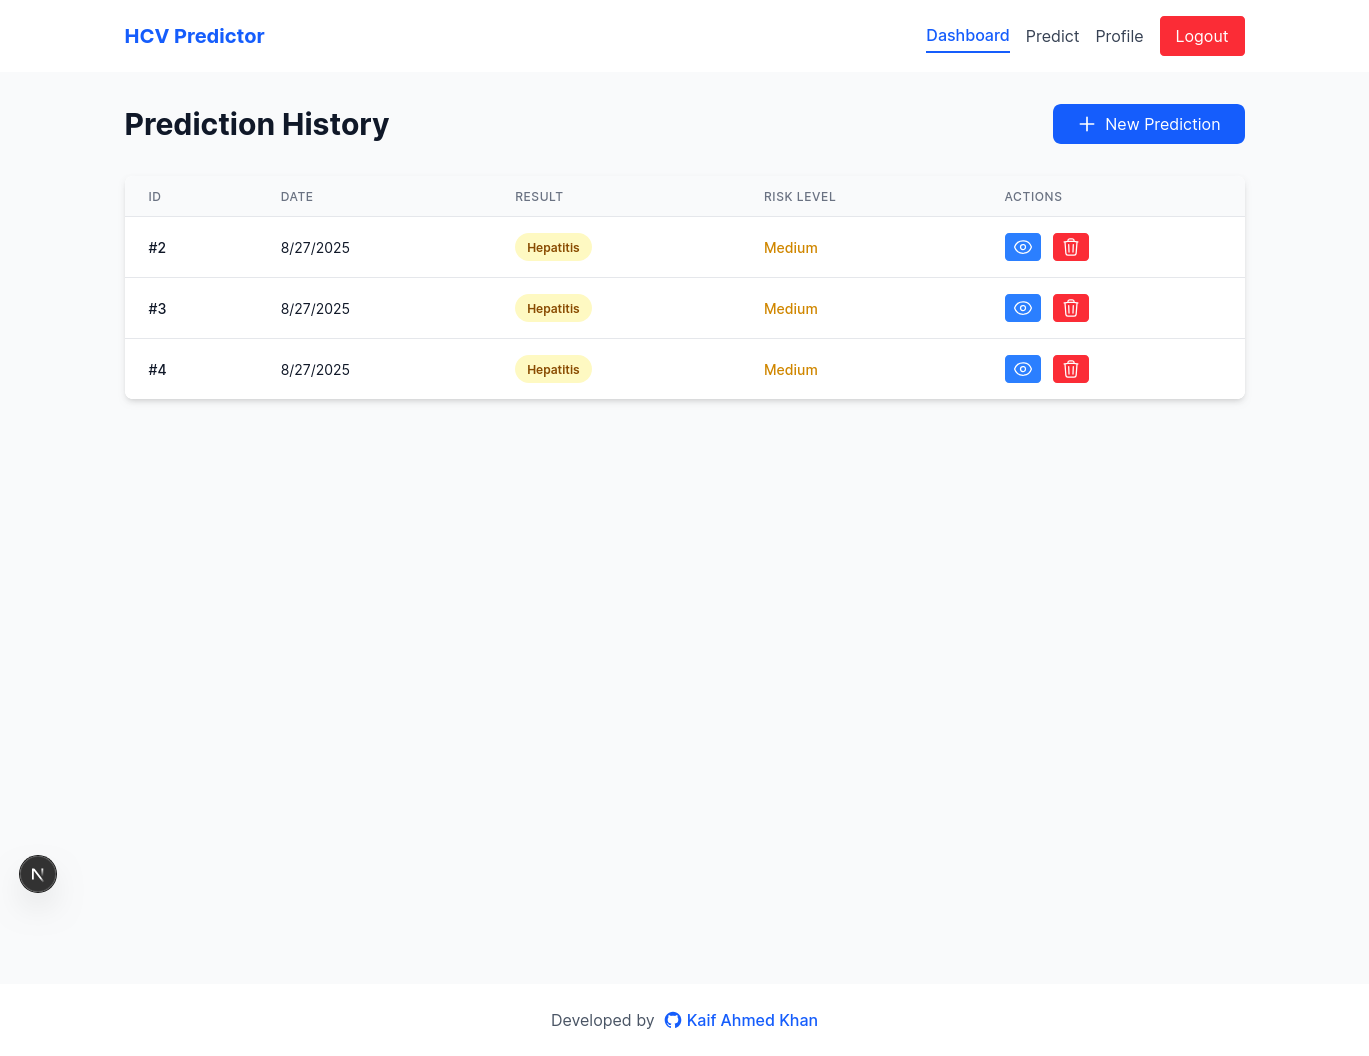
\includegraphics[width=\textwidth]{figures/site/dashboard.png}
    \caption{Prediction history in dashboard}
    \label{fig:dashboard}
  \end{subfigure}
  \begin{subfigure}{0.5\textwidth}
    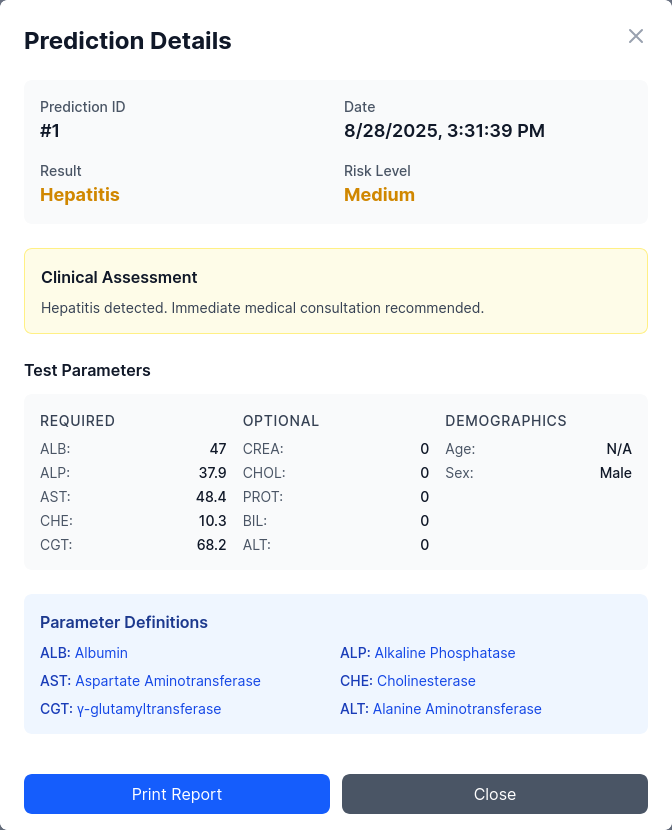
\includegraphics[width=\textwidth]{figures/site/details.png}
    \caption{Prediction details modal}
    \label{fig:details}
  \end{subfigure}
  \caption{Prediction system and prediction history in dashboard.}
  \label{fig:image2}
\end{figure}

\begin{figure}[htbp]
  \begin{subfigure}{0.5\textwidth}
    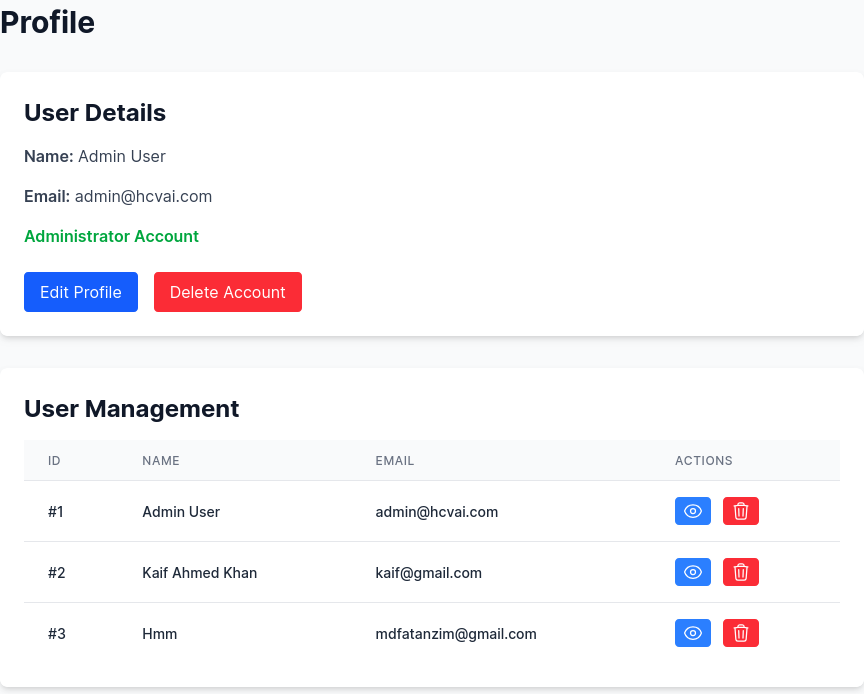
\includegraphics[width=\textwidth]{figures/site/admin.png} 
    \caption{Admin profile page}
    \label{fig:profile}
  \end{subfigure}
  \begin{subfigure}{0.5\textwidth}
  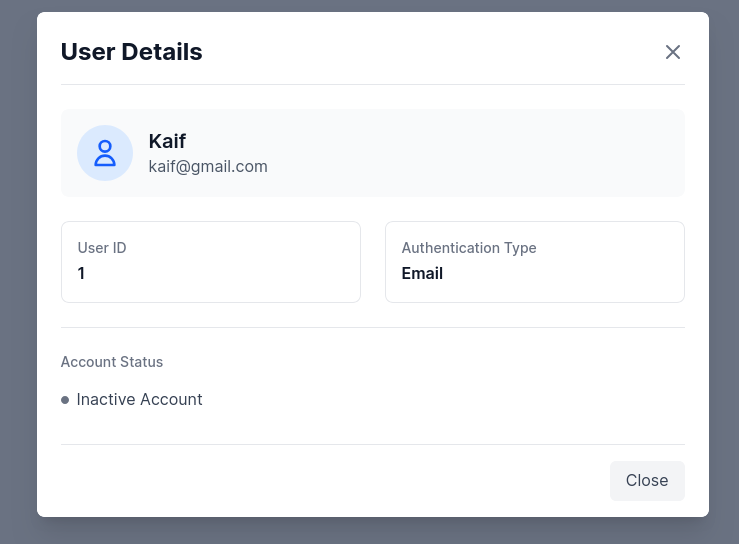
\includegraphics[width=\textwidth]{figures/site/user-details.png}
    \caption{User details modal}
    \label{fig:userdetails}
  \end{subfigure}
  \begin{subfigure}{0.5\textwidth}
    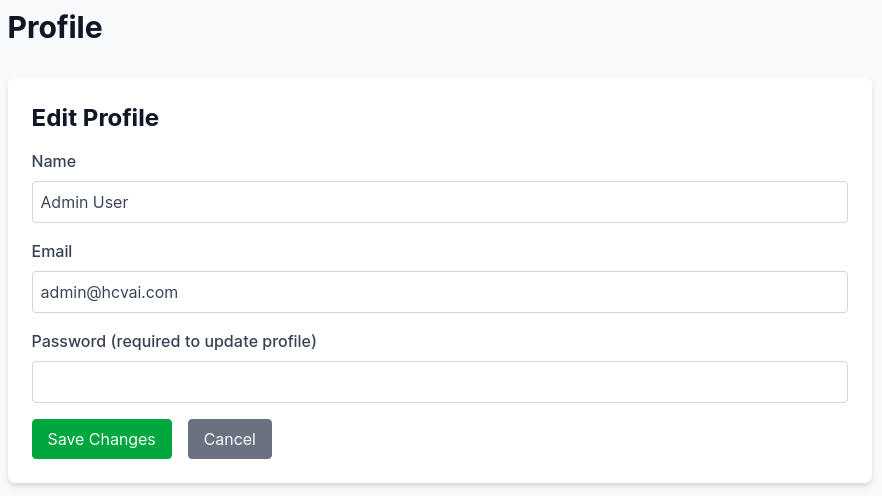
\includegraphics[width=\textwidth,height=6cm]{figures/site/edit.png}
    \caption{Edit profile details}
    \label{fig:edit}
  \end{subfigure}
  \begin{subfigure}{0.5\textwidth}
    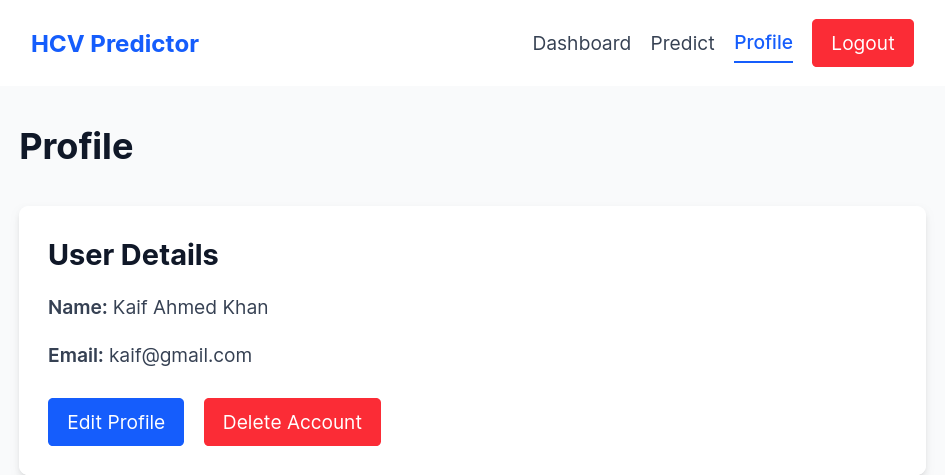
\includegraphics[width=\textwidth, height=6cm]{figures/site/normal.png}
    \caption{Non-admin profile page}
    \label{fig:detail}
  \end{subfigure}
  \caption{User Management. Link: https://172.104.62.100/profile}
  \label{fig:image3}
\end{figure}

\begin{figure}[htbp]
  \begin{center}
    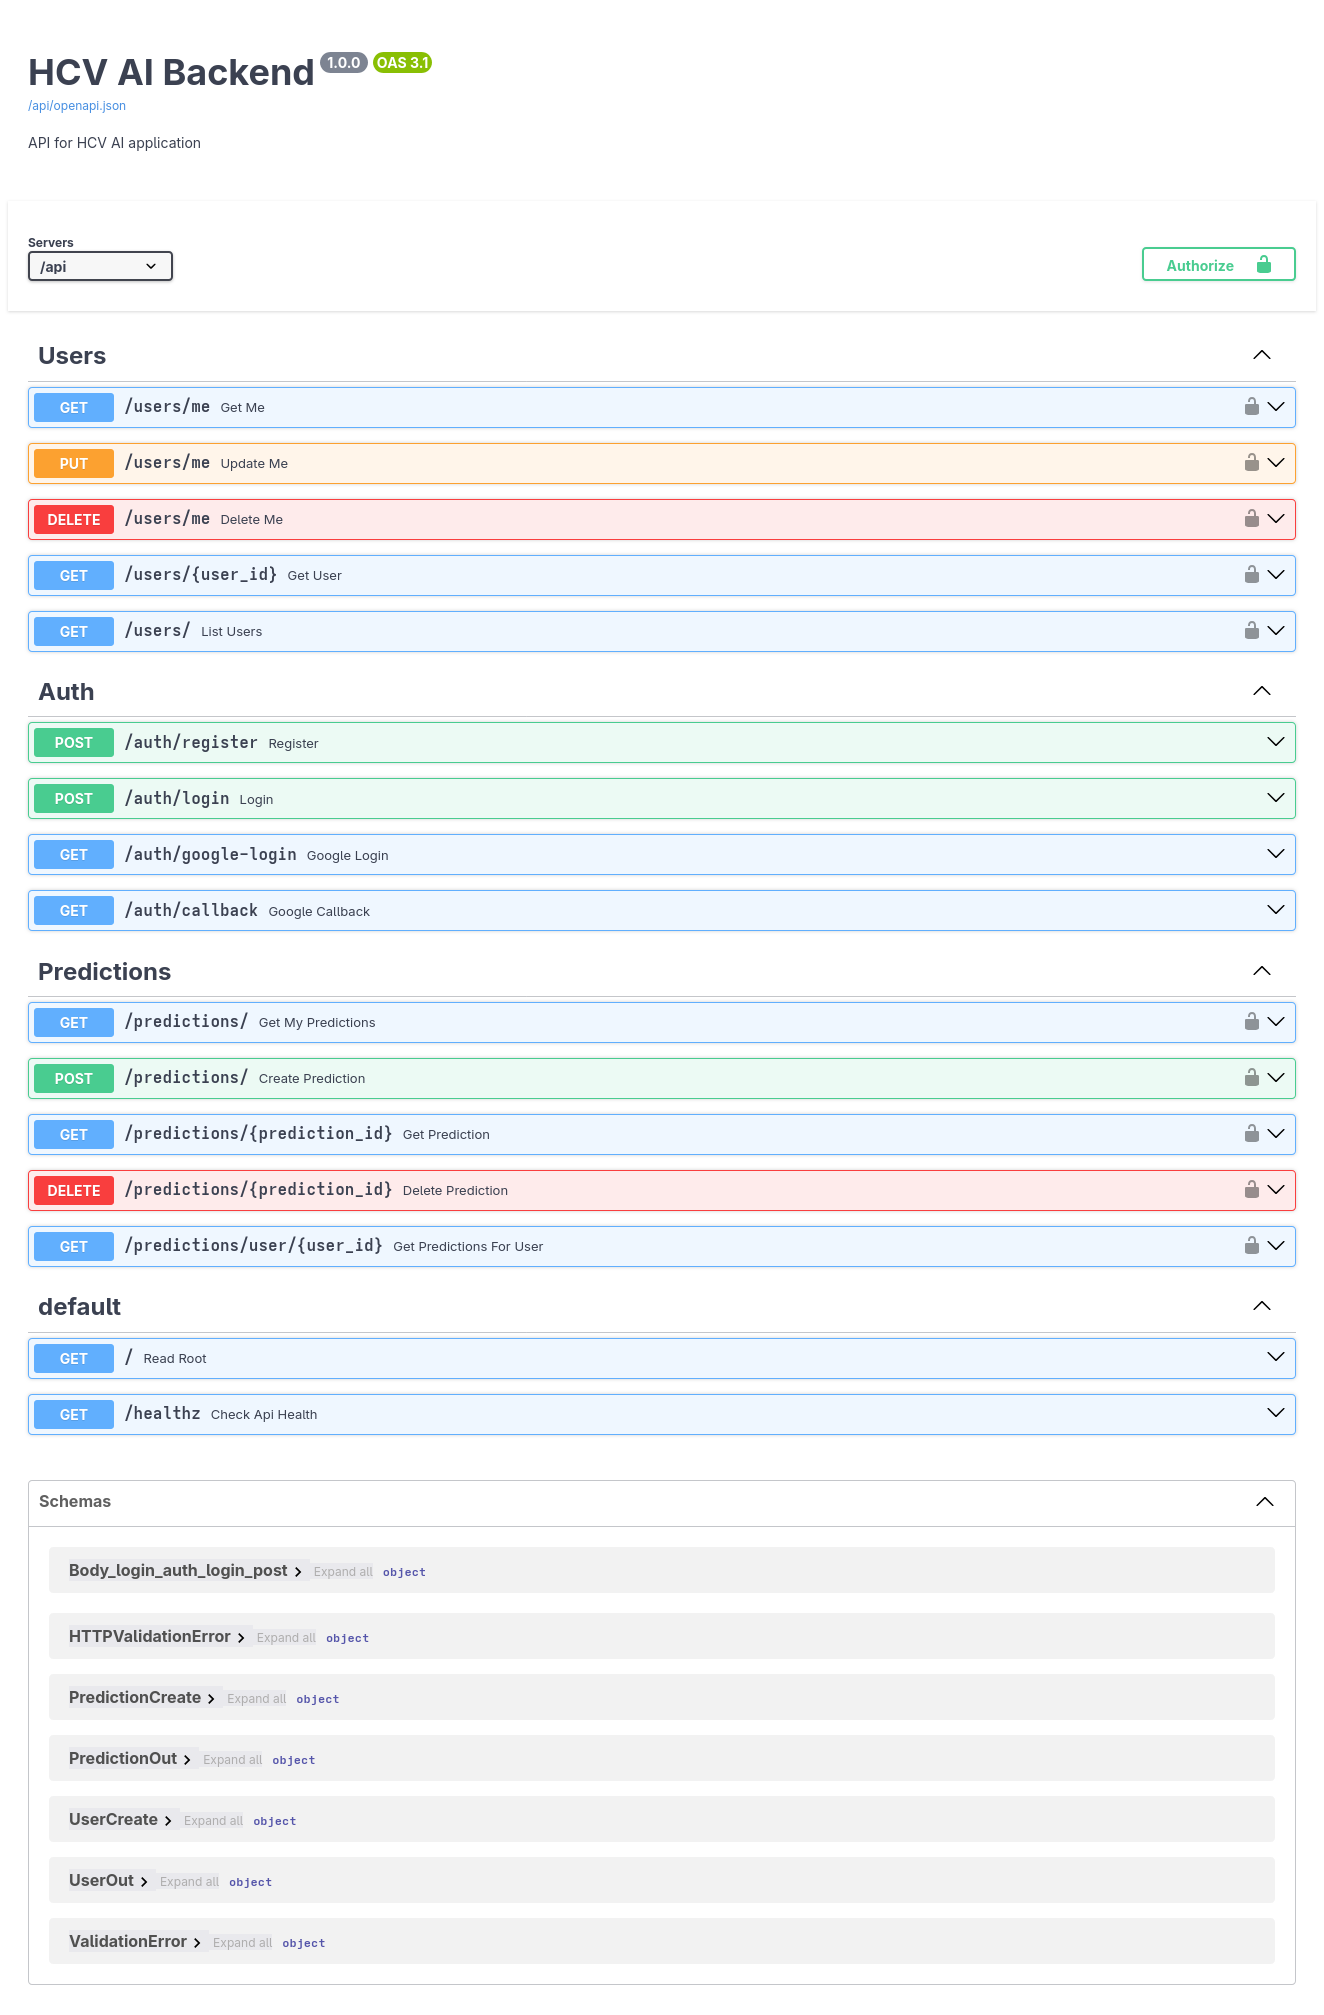
\includegraphics[width=\textwidth]{figures/site/backend-api.png}
  \end{center}
  \caption{FastAPI backend documentation @ \url{https://172.104.62.100/api/docs}}\label{fig:backend-api}
\end{figure}


\subsection*{User Management}
\begin{itemize}
    \item User registration and login system with SQLite database authentication.
    \item Role-based access control: Patients (users) and Admins.
    \item Secure storage of user information.
\end{itemize}
\subsection*{Prediction System}
\begin{itemize}
    \item Input form for blood report data (patient submits laboratory values).
    \item Pretrained machine learning model processes the input.
    \item Prediction of HCV stage (4 classes: 0--3).
    \item Prediction result is displayed instantly to the user.
\end{itemize}

\subsection*{Prediction History}
\begin{itemize}
    \item Patients can view their own previous predictions.
    \item Admins can view all users' predictions for monitoring and analysis.
\end{itemize}

\subsection*{Database Integration}
\begin{itemize}
    \item SQLite database with two main tables:
    \begin{itemize}
        \item \textbf{Users Table}: Stores user credentials and profile information.
        \item \textbf{Predictions Table}: Stores patient input, prediction results, and timestamps.
    \end{itemize}
\end{itemize}

\subsection*{Security and Roles}
\begin{itemize}
    \item Authentication system for both patients and admins.
    \item Role-specific permissions (patients see only their own data, admins see all data).
\end{itemize}

